%!TEX root = thesis_cgo.tex
\chapter{Introduction}

\epigraph{Everything existing in the universe is the fruit of chance and necessity.}{Democritus}

Molecular machines are assemblies of proteins that interact in a coordinated manner to solve a biological problem. These biological problems, such as coordinating chromosome separation during cell division, \todo{get more examples}, etc.  cover all processes essential to life. Given the necessity for survival in the face of ever changing environments, evolution has produced a large diversity of intricate molecular mechanisms for solving these problems in a flexible and robust manner. A machine that functions properly only under unchanging conditions and inputs is not likely to survive in a biological context. Therefore, at the core of each of those processes are highly complex networks of protein interactions that are able to assemble, communicate, coordinate, self-regulate and self-correct in order to accomplish the necessary task reliably. \todo{maybe put DNA example in next paragraph}For example, the vital process of DNA replication is executed by a large multitude of proteins that each contribute to the process of copying the genome. The replication machinery must read environmental queues for initiating replication at the correct time, while complex combinatoric signalling networks ensure that DNA replication unfolds in a processive manner, enzymatic components perform physical work by unwinding the DNA strand for copying, and others communicate with the DNA repair machinery to correct copying errors and avoid harmful mutations. It is clear that solving this biological problem requires the ability of participating proteins to interact with many different partners and mediate many different processes.  

The way proteins are able to control interactions and drive function is through the conformational arrangement of their backbones which is encoded in each protein's amino acid sequence. Specific spatial arrangements of peptide chains, also known as protein structure, allows for specific interactions between proteins to assemble molecular machines, recruit necessary factors and mediate necessary chemical reactions. \todo{include figure of yeast $\gamma$-tubulin structure to illustrate stable vs IDP} Since the 1950s when the first X-ray crystallography protein structure was solved, we have learned a great deal about how 3D architecture and motions of the chains give rise to protein function. By capturing various conformations of folded protein domains, we have been able to infer that motions between structural conformations is the main element of control in protein function. For example, \todo{example of basic protein structure-rearrangement}. \figref{tub4}  However, it is important to note that X-ray crystallography only offers static pictures of protein structure, and provides information mostly the spatial arrangement of relatively large stable domains in proteins. It therefore became a long standing dogma that the stable 3D folds of a protein chain dictate a protein's function. Yet, as we saw with DNA replication, molecular processes are incredibly complex, and a single protein often has to play many roles, interact with various different partners and be able to do so in a rapid and controllable manner. It is therefore unlikely that such large scale and consequently slow structural motions can account for all of the precise and rapid control we observe in biological systems. A static description of proteins is not sufficient to explain the degree of functional flexibility and control that we observe. This leaves us with the questions of how can the same protein fulfill multiple functions and engage in many different interactions? How can molecular machines offer such precise control of functionality while counting only on a static architectures? The broad aim of this thesis is therefore to improve our understanding of the physical mechanisms underlying the functional complexity of molecular machines.



\section{Disorder in proteins}

One potential source of plasticity can be found when looking more closely at proteins we find that the majority contain significant levels of structural flexibility, also termed intrinsically disordered regions, or proteins (IDPs). \todo{fix this sentence}.  IDPs are segments of protein, or entire proteins, that do not natively adopt any stable conformation or fold but are often functionally active and thus do not follow the classical structure-function paradigm. \footnote{We will use the term IDP loosely to denote any unstructured protein element. Some works make the distinction between IDP and IDR where an IDR is an intrinsically disordered region and is not a full protein. There will be instances in the text where we will use IDR in this way.}Instead, IDPs are highly dynamic by nature and are able to rapidly sample a wide range conformations in an almost stochastic manner. This flexibility offers the protein access to a vast pool of possible conformations with which to fine-tune and diversify its function. It can then be said that IDP function lies in the \lq absence\rq of structure. The lack of structure in IDPs can be explained by the characteristically low sequence complexities, an enrichment for polar and charged residues over large hydrophobic amino acids which tend to favour rigid folding. 

For a long time, these types of protein element were overlooked in favour of studying stable folding patterns. In the case of IDRs, IDRs were thought to act simply as flexible linkers between structural domains without any  function or their own. This was also due in part to the fact that the main tool being used for structural biology, X-ray crystallography, fails to detect patterns in unfolded chains, making it difficult to study highly dynamic elements in protein such as IDPs. Techniques that do produce information on dynamics such as NMR only developed for proteins until much later; the first protein structure solved by X-ray crystallography was in 1958 and it was not until 1984 when the first protein structure was solved using NMR. Likewise, computational tools to study protein dynamics {\it ab initio}, such as Molecular Dynamics (MD) were greatly limited by shortcomings in processor power. However, with large advances in experimental and computational techniques in recent years, we have been able to study the dynamic properties of IDEs in great detail, and have found that they play key roles in the functioning of molecular machines. 


\begin{figure}
\centering
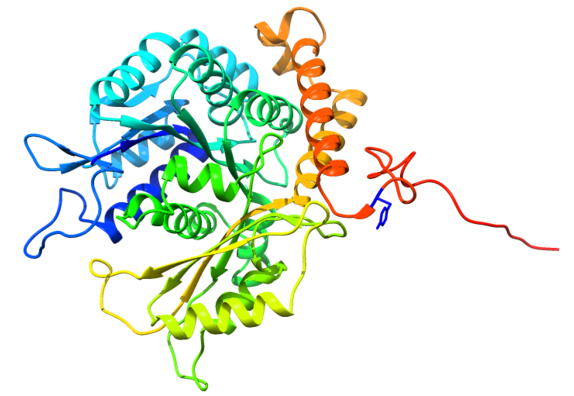
\includegraphics[height=0.3\textheight]{figures/tub4_tyr.png}
\caption{Homology model}
\end{figure}

\section{Physical mechanisms of IDP function in cellular machines}

Given that disorder in proteins is so prevalent it is not surprising that IDPs have been implicated in a multitude of cellular processes through NMR and mutational studies. These processes include signalling, cell cycle control, transcription, translation, ribosome assembly, chromatin organization, microtubule assembly/disassembly, etc. Mutations in IDPs have been shown to be involved in several disease phenotypes.  Interestingly, it has been shown that viral proteins use IDPs in their proteins to hijack cellular proteins and use the flexibility of IDPs to mimic host proteins and recruit host cellular machinery in order to propagate.\cite{davey2011viruses} An interesting hypothesis that came from these observations is that viral proteins use IDPs to make efficient use of their smaller genomes and obtain a greater range of function from the limited number of proteins in their genomes. It is now clear that IDPs, through their lack of structure, are an important adaptive feature allowing the functional complexity and robustness we observe in molecular machines. \\

In this section we will give a brief account of some of the physical mechanisms of IDP function that have been described in the literature. \\

{\it Phosphorylation}

A key aspect of dynamic control is the ability to modulate function in a precise and reversible manner.  The cell needs to be able to induce and inhibit interactions in a time and space dependent manner. To solve this problem, the cell harnesses the structural malleability of IDPs by coupling it with post translational modifications, most commonly, phosphorylation. Phosphorylation is the reversible addition of a phosphate group, which carries a negative charge, to one a tyrosine or serine amino acid by a kinase enzyme. The reverse reaction is catalyzed by enzymes called proteases which remove the phosphate group. The addition of a phosphate group introduces the potential for hydrogen bonding with itself and with other targets, and alters the electrostatic environment of the IDP. This change can therefore bias the stochastic conformational sampling of the IDP in a particular direction, and because it is reversible, it acts as a structural switch which can then be used to modulate a large range of interactions. Not surprisingly, it has been seen in many studies that IDPs are prime targets for phosphorylation {\it in vivo}.  The use of phosphorylation as an information carrier has been described in various cellular systems. For example, in cell cycle control, a specific temporal sequence of interactions has to be enforced. Therefore, the sequential phosphorylation of a single target can modify the affinity for the same target to the subsequent target in the pathway. Phosphorylation can also be used to enforce thresholds, where to avoid the negative impact of interactions by coincidence, certain interactions will only be activated once an IDP has achieved a certain number of phosphorylations.   ... \\ \todo{insert examples of phosphorylation in combinatorial, information carrying, etc.}

{\it Disorder-Order transitions}

The best explored physical mechanism of IDP function is the fold-on binding paradigm. In this case, IDPs in the free form are unstructured, and when they encounter their binding target, they undergo a folding transition (disorder to order) to form a stable complex. The lack of structure in the unbound state allows the the IDP to recognize multiple targets, and it allows the binding to be inducible instead of constitutive. A well studied example of this kind of mechanism is the binding of the transcriptional activator protein CREB and its co-activator CPB. An IDR in CREB known as KID mediates binding to CPB where upon binding, the IDP folds into a pair of helices. However, this binding process is not favoured spontaneously due to loss of entropy induced by folding. \footnote{If we consider the expression for Gibbs free energy, $\Delta G = \Delta H - T\Delta S$, where $\Delta H$ is the change in enthalpy, or heat energy available to the system, and $\Delta S$ is the entropy, or degree of disorder/conformational freedom available to the system. If we define our system as a protein chain, we see that a decrease in entropy which can be brought upon by the ordering of a structure will result in a positive $\Delta G$ thus making the reaction energetically unfavourable. This loss of entropy, or conformational freedom, can be overcome by a release of heat, or a sufficiently negative $\Delta H$ component which can tip the energetic balance toward $\Delta G < 0$. One might say that the decrease in entropy in the protein would be in violation of the second law of thermodynamics which states that all systems tend toward an increase in entropy. However, a reaction with a negative $\Delta H$, in other words, a reaction releasing heat will cause an increase in entropy to its surrounding environment. In the case of protein, the process of folding will reduce generally the entropy of the protein, but if the folding has a negative $\Delta H$ it will release heat and thus increase the entropy of the water molecules surrounding it.}However, when the KID is phosphorylated, the phosphyl group interacts with CPB by forming hydrogen bonds which result in a negative enthalpic change that compensates for the loss of entropy and thus makes the folding reaction favourable. Because of the inducible nature of this interaction, CPB is able to also interact with other co-factors, which has been reported in the literature. \cite{radhakrishnan1997solution} This is an example of how even though the association state of the IDP is ordered, without the intrinsic disorder of the unbound state, the high entropy of IDPs acts as a barrier for binding which can be overcome to promote interactions in a controllable manner. \\


\pagebreak

{\it \lq Fuzzy\rq interactions}

\par Disorder to order transitions are not necessary for IDPs to confer functionality. There is a growing number of examples where IDPs are involved in functional interactions while remaining in a disordered state \cite{tompa2008fuzzy}. Such interactions have been labeled with the term \lq fuzzy\rq as they maintain a heterogenous conformational ensemble throughout their lifetimes. There exist various physical mechanisms by which fuzziness, or disorder, in binding interactions confers advantages to protein function. For example, binding interactions between an IDP and a target protein where the IDP is able to form alternate contacts with its binding target can help reduce the entropic cost of binding, as well as control the accessibility of different sites on the protein for modulating interactions with different targets. \cite{graham2001tcf4, fontes2000structural} IDPs can also play a role in interactions without making direct contacts with the binding partner.  By acting as flexible linkers for folded domains \cite{bhattacharyya2006ste5}, or as \lq antennae\rq for \cite{sigalov2004homooligomerization} recruiting further interactions and stabilizing the binding of folded domains through long range interactions \cite{zor2002roles, yu1994structural} \todo{paragraph feels too compact}

It is becoming increasingly evident that nature is able to harness disorder as an adaptive mechanism for control in protein-function. Flexibility in conformational state allows cellular processes to greatly expand the functional repertoire of proteins by allowing for rapid switch-like control over interactions, expanding the functional repertoire of proteins, and fine-tuning the kinetics of interactions.  It is due to all of these various physical mechanisms that the cell is able to carry out its complex tasks with such robustness and precision. Advances in this field have caused us to reconsider the paradigm of \lq one structure, one function\rq that has prevailed in structural biology for decades. However, this remains a relatively novel area of structural biology, and there still remain many unsolved physical mechanisms in IDPs.

\section{IDP function in the mitotic spindle}
 
In this section we will address the role of IDPs in controlling the function of the mitotic spindle. The mitotic spindle is a complex molecular machine composed of microtubules, force generators, effector proteins, chromosomes, and numerous effector molecules which act in a coordinated manner to accomplish the process of chromosome segregation during cell division. This process ensures that genetic material is transferred from the mother to the daughter cell in a timely manner and without errors which would in most cases result in lethality. Because cell division is a fundamental task in every cell's lifetime, the mitotic spindle has shares common design features throughout eukaryotes. The task of properly arranging and segregating chromosomes is effected ultimately by filament-like polymers known as microtubules which attach to chromosomes and physically pull the DNA to the daughter cell. In order to study the underlying mechanisms at play, we work with the mitotic spindle of the budding yeast {\it Saccharomyces cerevisiae} due to its minimal, yet highly conserved construction. 

\subsection{Microtubules}

Microtubules are constructed of alternating pairs, or dimers, of the globular proteins $\alpha$ and $\beta$ Tubulin. A cylindrical arrangement of tubulin dimers results in the formation of a rigid tube-like structure, which by growing, or polymerizing, or shrinking, depolymerizing, can effect force on a target. Microtubules are involved in a number of other functions, such as serving as roadways along which transport molecules can carry cargo, and forming the structural backbone of the cell. The spontaneous assembly of tubulin dimers in solution into a microtubule is heavily disfavoured. However, when free floating tubulins encounter pre-formed ring of tubulin molecules, the growth of a microtubule is greatly facilitated. In cells, this template is known as the $\gamma$-Tubulin Ring Complex ($\gamma$-TuRC) which is a ring-like structure of $\gamma$-Tubulin molecules held together by various other proteins known as $\gamma$-tubulin ring proteins (GRIPs). $\gamma$ tubulin shares a similar structure to $\alpha$ and $\beta$ tubulin and have been shown to act as nucleation templates for microtubules. Furthermore, structural rearrangements of the $\gamma$-TuRC have been shown to either facilitate and inhibit nucleation. 

\subsection{$\gamma$-Tubulin \& the $\gamma$-CT}

For many years, microtubule nucleation was though to be the sole function of $\gamma$ tubulin. However, in 2001, a mass spectrometry study of the yeast $\gamma$-Tubulin showed that the protein is phosphorylated {\it in vivo} at 9 sites. \todo{how many sites?} Several functional studies following up on the finding that $\gamma$-tubulin is regulated show that mutations altering phosphorylation sites, all of which lie in IDRs, have consequences on the organization and stability of microtubules but no effect on their nucleation.  

One of the best studied phosphorylation sites in $\gamma$-Tubulin is the heavily conserved Tyrosine (Y) 445 which lies in the disordered carboxyl terminal tail of $\gamma$-Tubulin (\gct).  The \gct{} is defined as the final 35 residues in the C-terminal portion of $\gamma$-Tubulin, where the folded globular domain ends. Substitution of an Aspartic Acid (D) residue in the place of Y445, making the Y445D mutant, results in slow growing cells with unstable and misaligned mitotic spindles. The aspartic acid substitution is used as a controllable means for recreating the electrostatic environment of a phosphate group by introducing a negative charge. These findings suggest that $\gamma$-Tubulin is playing a role outside of its canonical function of nucleation and is coordinating the dynamics of the mitotic spindle. The coupling of post-translational modifications (PTMs) to the C-terminal tails o tubulins has been described in the $\gamma$-tubulin orthologues $\alpha$ and $\beta$ tubulin. Specific combinations of PTMs on the tubulin tails act as a \lq tubulin code\rq for recruiting motor proteins and microtubule associated proteins to the microtubule lattice. A similar code has not yet been described for $\gamma$-Tubulin.  While the functional importance of phosphorylation and IDRs in $\gamma$-Tubulin is becoming increasingly clear, the physical mechanisms by which local modifications at IDRs can have global impacts on the large molecular machine remain unstudied. 
 
 \section{Experimental question}
 
 We hypothesize that the addition of a negative charge at the position Y445 in the \gct{} alters the conformational sampling of the disordered tail in such a was as to be able to regulate the function of the complex.  
 
 \section{Approach}
 
In order to detect the rapid changes in conformational sampling, we use a powerful computational technique known as Molecular Dynamics (MD) simulations. We will be simulating the dynamics of the \gct{} in isolation as well as in the presence of the entire $\gamma$-Tubulin protein. \todo{should I bring up NMR here?}

\todo{Notes from jackie: keep REMD in discussion as possible method. Tony says REMD more for overcoming enthalpies not entropic barriers so not good for IDPs. Need to sample for longer to see changes.}
 
 
 
 
 